\section{Jenkins \emph{Build}}
\label{sec:jenkins-build}



\subsection{Stage Prepare}

In diesem Build-Schritt werden alle Vorbereitungen für den eigentlichen Build getroffen. Es werden Variablen für \emph{Stash} und \emph{Unstash} angelegt, um das Projektverzeichnis zwischen den Steps/Pods zu verschieben. Weiters wird das aktuelle Repository verifiziert und eine Prüfsumme abgefragt.

\begin{minted}{groovy}
stage('Prepare') {
  println "Preparing the build..."
  STASH_GIT_REPO="git-repo"
  STASH_BUILD="build-result"

  println "Stashing git repo..."
  dir('../workspace@script'){
    GIT_REF = sh returnStdout: true, script: 'git rev-parse --verify HEAD'
    stash name: STASH_GIT_REPO, includes: '**/*'
  }
  println "Stashed  git repo: 'git-repo'"
  println "Prepared  the build"
}
\end{minted}

\begin{figure}[H]
	\centering
	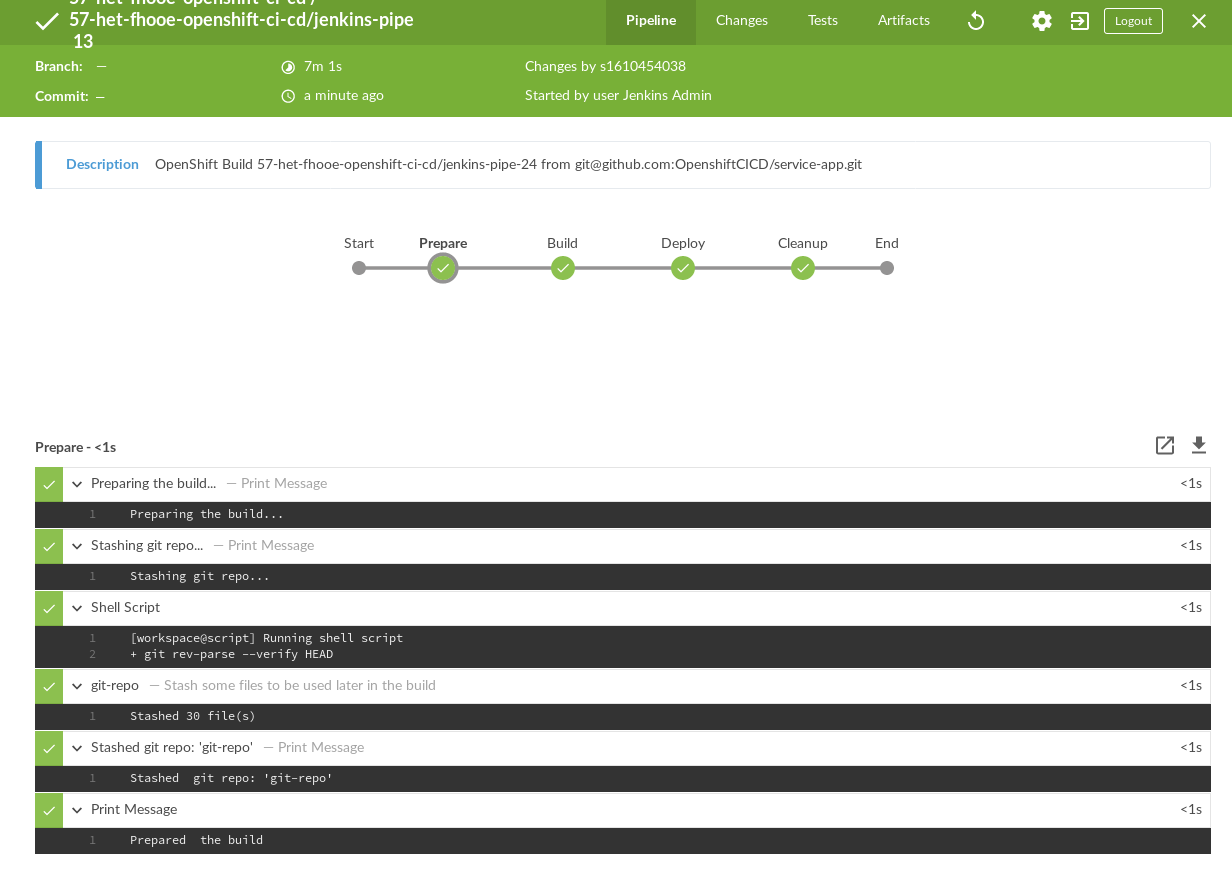
\includegraphics[scale=0.4]{image/jenkins-prepare.png}
	\caption{Prepare Build Server}
	\label{fig:architecture}
\end{figure}

\pagebreak

\subsection{Stage Build}

Der eigentliche \emph{Build} findet in einem Pod, d.h. in einem \emph{Build-Slave}, der extra dafür gestartet wird, statt. In diesem Fall wird ein \emph{Gradle-Build-Slave} gestartet, die \emph{Sourcen} werden mittels \emph{./gradle} gebaut und danach wird der \emph{Build-Slave} zerstört. Zusätzlich werden noch Umgebungsvariablen an Gradle übergeben, welche in den Build-Targets genutzt werden, um z.B. Abhängigkeiten aus einem lokalen Nexus-Repository zu laden.

\begin{minted}{groovy}
stage('Build') {
  NEXUS_USER="${env.NEXUS_USER}"
  NEXUS_PASSWORD="${env.NEXUS_PASSWORD}"
  NEXUS_MIRROR_URL="${env.MAVEN_MIRROR_URL}"
  MAVEN_REPOSITORY_URL="${env.MAVEN_REPOSITORY_URL}"

  podTemplate(name: 'jenkins-slave-gradle',
        cloud: 'openshift', containers: [
    containerTemplate(name: 'jnlp',
            image: 'ci/jenkins-slave-gradle', resourceRequestCpu: '500m', 
            resourceLimitCpu: '4000m', resourceRequestMemory: '1024Mi', 
            resourceLimitMemory: '4096Mi', slaveConnectTimeout: 180)
  ]) {
    node('jenkins-slave-gradle'){
      container('jnlp'){
        println "Unstashing '${STASH_GIT_REPO}'..."
        unstash STASH_GIT_REPO
        dir('\\complete') {
          echo sh(returnStdout: true, script: "gradle 
          -PnexusUsername=$NEXUS_USER -PnexusPassword=$NEXUS_PASSWORD 
          -PmirrorUrl=$NEXUS_MIRROR_URL 
          -PrepositoryUrl=$MAVEN_REPOSITORY_URL build")
        }
        println "Built  with gradle"
          
        println "Stashing the workspace..."
        stash name: STASH_BUILD, includes: '**/*'
        println "Stashed  the workspace"
      }
    }
  }
}
\end{minted}

\pagebreak

\subsection{Stage Deploy}

Der Trigger \emph{OpenShiftBuild} führt das Äquivalent zum Aufruf des Befehls oc start-build aus, bei dem die Build-Protokolle in Echtzeit an die Ausgabe des Jenkins-Plug-ins ausgegeben werden können. Zusätzlich zur Bestätigung, ob der Build erfolgreich war oder nicht, kann dieser Build-Schritt optional prüfen, ob die Deployment-Configs sogenannte Image-Change-Trigger für das von der Build-Config erzeugte Image haben. Wenn solche Deployment-Configs gefunden werden, werden diese  analysiert, um festzustellen, ob sie durch eine Imageänderung ausgelöst wurden. Dabei wird das vom aktuell ausgeführten Replication-Controler verwendete Image mit dem Image verglichen, das von seinem unmittelbaren Vorgänger verwendet wurde.

\begin{minted}{groovy}
stage('Deploy') {
  // Set app version on app build config
  echo sh(returnStdout: true, 
              script: "oc env buildconfigs/spring-boot VERSION=1.0.0")

  // Trigger the build config with the new version
  openshiftBuild(buildConfig: 'spring-boot', 
                       showBuildLogs: "true", 
                       checkForTriggeredDeployments: "true")
                       
   // Verify successful deployment
   openshiftVerifyDeployment(deploymentConfig: 'spring-boot', 
                                           replicaCount: "1", 
                                           verifyReplicaCount: "true",
                                            waitTime: "30000")
}
\end{minted}

\begin{figure}[H]
	\centering
	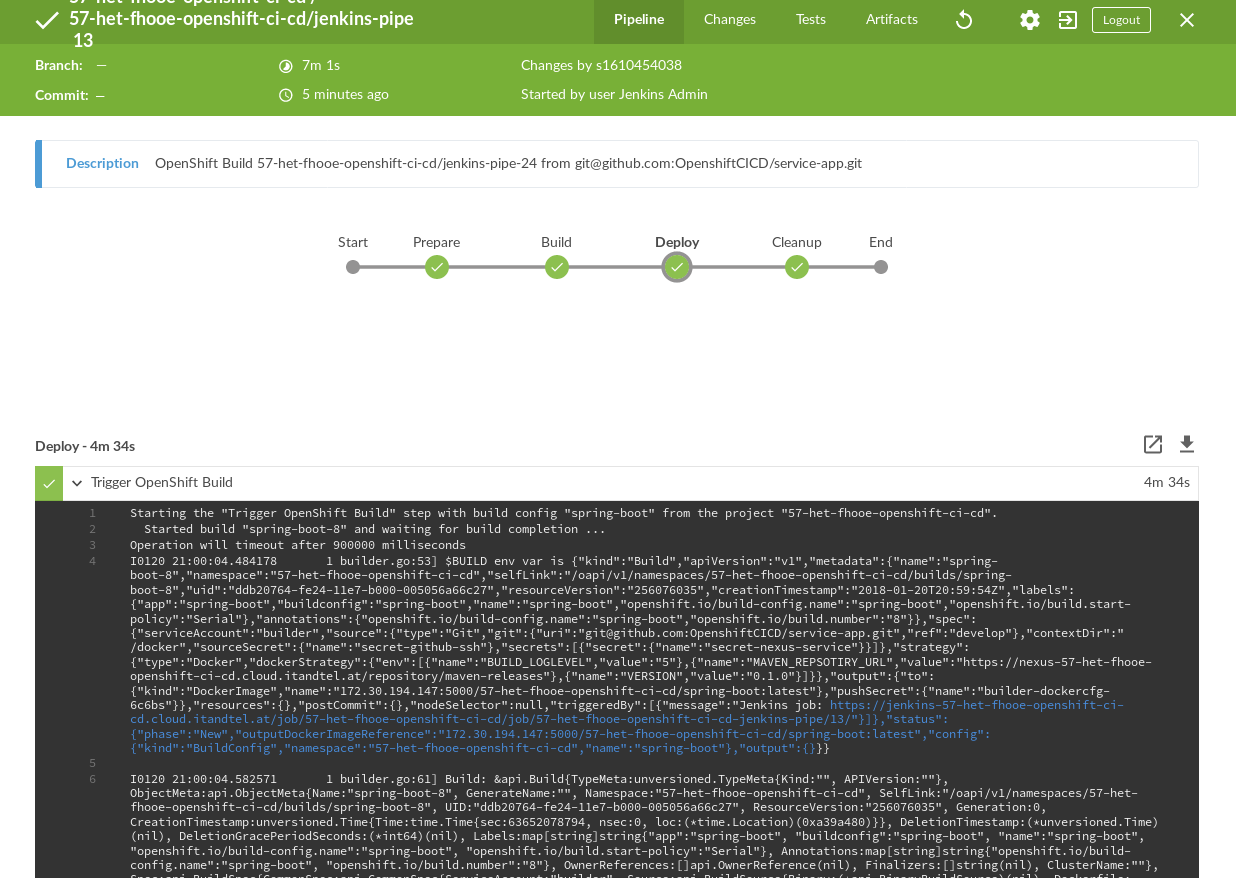
\includegraphics[scale=0.3]{image/jenkins-deploy.png}
	\caption{Deploy Build}
	\label{fig:architecture}
\end{figure}